\chapter{Application}
\label{chap:application}
The GNN model introduced in \autoref{chap:gnn} will be benchmarked on various datasets in the following chapters. All reference data was calculated using the 6-31G(2df,p) basis at theory level B3LYP. \\

Models will be evaluated by their iteration count till convergence, the energy difference from the converged solution the DIIS error (see \autoref{eq:diis_error}) and RMSE. The inference time of all models, just a few milliseconds, is roughly three orders of magnitude shorter than that of a typical DFT calculation, and can therefore be regarded as negligible. This performance holds across all applications discussed below.

\section{QM9 - \ch{C7H10O2} Isomers}
\label{sec:qm9_isomers_benchmark}
There are 6095 structural isomers of \ch{C7H10O2} in the QM9 dataset (see \autoref{sec:dataset}). Analogous to the trials performed in \autoref{sec:further_trials_mlp}, we will train and validate on a randomly drawn sample of 500 isomers\footnote{using \textsc{scf\_guess\_datasets} (see \autoref{subsec:gnn_normalization})}. This reduction is necessary to make training and hyperparameter-tuning feasible in the scope of the thesis. Contrary to the full matrix prediction schemes in \autoref{chap:fock_matrix_predictions}, we employ sub-matrix predictions and reconstruct the full matrix thus making the actual number of samples significantly higher. Per molecule sample we get 7, 10 and 2 samples for \ch{C}, \ch{H} and \ch{O} respectively, totalling 3500 \ch{C}, 5000 \ch{H} and 1000 \ch{O} samples. This already provides some rotational variability. Additional rotations can be introduced through data augmentation during training to develop a model that is agnostic to rotation when predicting density.\\

\subsection{Initial training}
\label{subsec:qm9_isomers_initial}
%! refer to MGNN_6-31G_NO_AUG_07_07_manual_ref.pth
To gauge the performance of the GNN devised in \autoref{chap:gnn} manual runs were performed during development. Hyperparameters were set according to \autoref{tab:init_hparams}. 

\begin{table}[H]
    \centering
    \caption[Hyperparameters - initial MGNN training (manually selected)]{Hyperparameters used for the initial MGNN training (manually selected)}
    \label{tab:init_hparams}
    \begin{tabular}{ll ll}
        \toprule
        \textbf{Hyperparameter} & \textbf{Value} & \textbf{Hyperparameter} & \textbf{Value} \\
        \midrule
        Hidden dimension & 256 & Msg. passing rounds & 4 \\
        MsgNet layers & 3 & MsgNet dropout & 15 \% \\
        Batch size & 16 & Grace period & 10 epochs \\
        Target & Density matrix & Loss function & MSE (block-wise) \\
        Learn rate (initial) & $2.68 \times 10^{-3}$ & Weight decay & $1.78 \times 10^{-5}$ \\
        Edge threshold & 3 \AA & Data augmentation & No \\
        \midrule
        Learn rate factor & 0.5 & Learn rate patience & 3 epochs \\
        Learn rate threshold & $10^{-3}$ & Learn rate cooldown & 2 epochs \\
        Learn rate min & $10^{-6}$ & — & — \\
        \bottomrule
    \end{tabular}
\end{table}
Note, that this initial run did not use data augmentation and thus trained on 400 samples (corresponding to our default data split of 80\% / 10\% / 10\%). The grace period, time without improvement, was set to 10 epochs to allow the learning rate scheduler sufficient time to take effect and for potential improvements to manifest thereafter.\\
Training and validation losses both monotonically decrease up to around epoch 30 as can be seen in \autoref{fig:initial_train_qm9_isomers}. While the loss on the validation set plateaus rather early, training loss decreases throughout the training process. 

\begin{figure}[H]
    \centering
    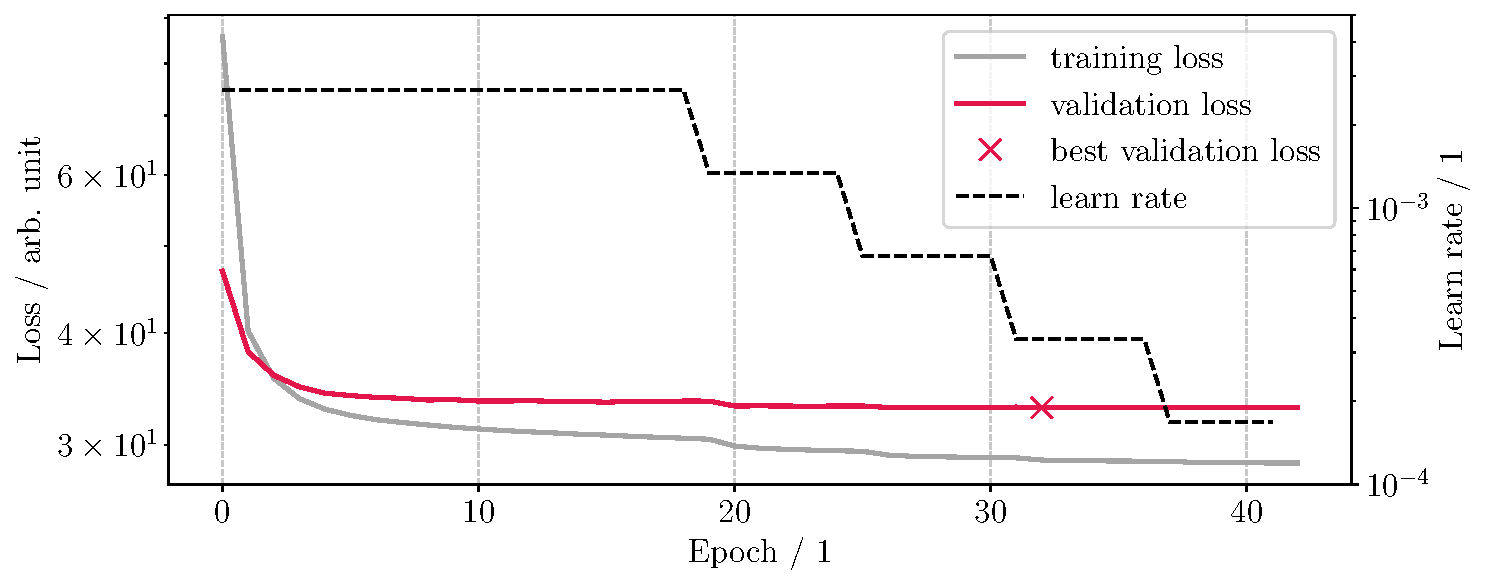
\includegraphics[width=\textwidth]{../fig/gnn/MGNN_6-31G_NO_AUG_07_07_manual_ref_train_val_loss.pdf}
    \caption[Initial GNN loss on QM9-isomers]{Initial GNN training / validation loss and corresponding learn rate per epoch on QM9-isomers.}
    \label{fig:initial_train_qm9_isomers}
\end{figure}
Both losses are further pushed down following learn rate decreases. This run produced the best model in epoch 33 with a validation loss of $33.00$ and a training loss of $28.83$ indicating slight overfitting which is to be expected especially without data augmentation in the training samples. The performance of the model $\text{GNN}_\text{initial}$ on the test set is compared to other models and guessing schemes in \autoref{tab:qm9_isomers_test_overview}. 



\subsection{Hyperparameter tuning}
\label{subsec:qm9_isomers_hyperparamtuning}
Generally, one uses the validation loss as a benchmark to select the best model from a hyperparameter run. While we will also prefer models with lower loss, we must be very careful not to select models which look good on paper but perform worse due to the lack good correlation between MSE and iteration count. For this reason, we will base our hyperparameter search on the $\text{GNN}_\text{initial}$ model and explore in a structured way. 

\textbf{Data augmentation}\\
$\text{GNN}_\text{initial}$ already performed quite well in terms of iterations without using any data augmentation. One might argue that there is already some data augmentation baked into the train set due to the different orientations of atoms in various molecules. 
\begin{figure}[h]
    \centering
    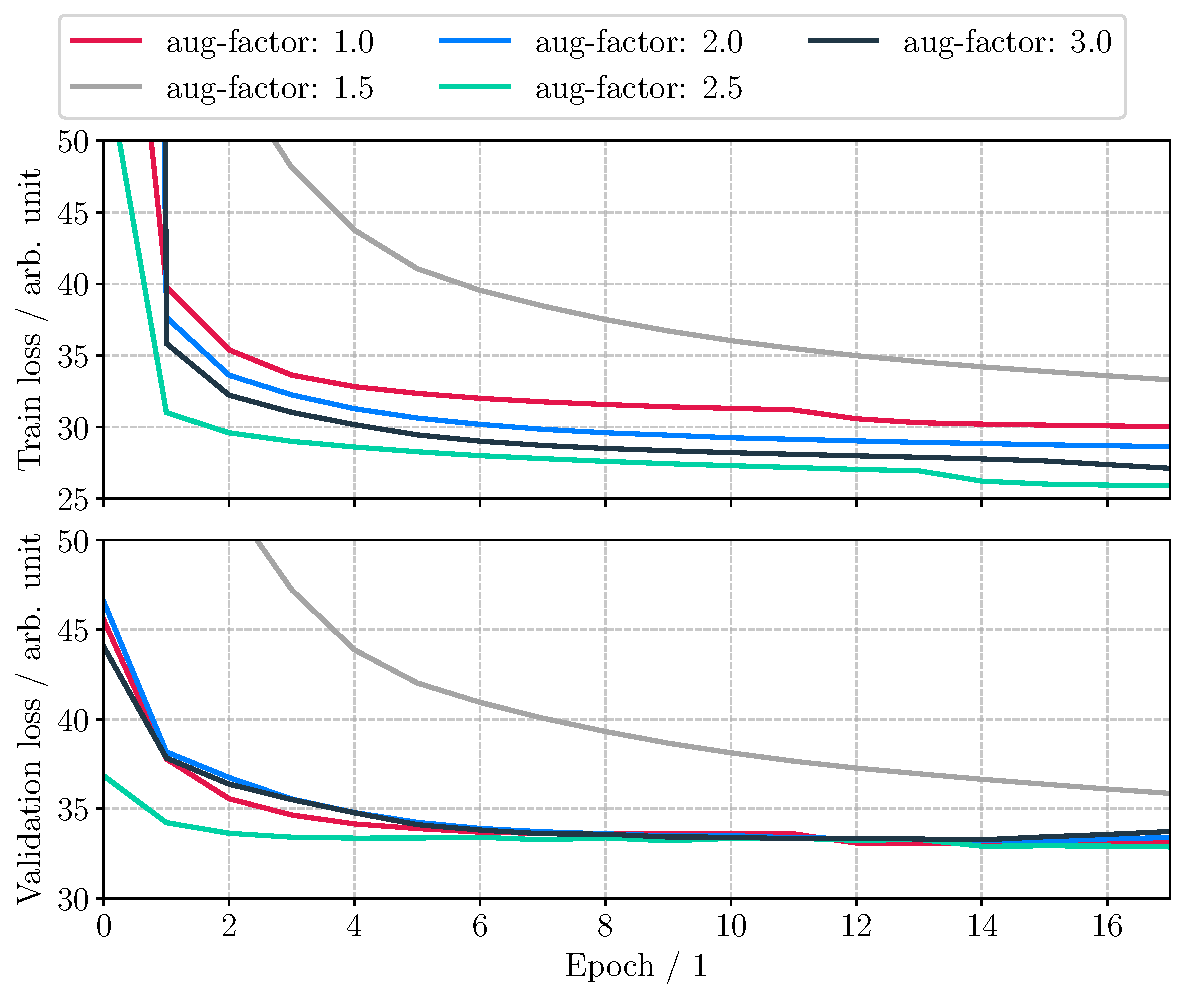
\includegraphics[width=0.75\textwidth]{../fig/application/aug_train_val_loss.pdf}
    \caption[GNN loss for different augmentation factors on QM9-isomers]{GNN loss for different data augmentation factors on QM9-isomers. All other hyperparameters are kept as in \autoref{tab:init_hparams}.}
    \label{fig:loss_hyper_qm9_isomers}
\end{figure}
Comparing the training and validation loss between different augmentation factors in \autoref{fig:loss_hyper_qm9_isomers} shows no clear trend regarding the choice of the augmentation factor. While a factor of $2.5$ initially outperforms no augmentation and other factors, they all converge in validation towards the end. 
Investigating different metrics on the test set in \autoref{tab:qm9_isomers_data_aug_hyperparam} does not yield conclusive insight. Our initial model has the best performance in terms of iterations. However, other models do not fall far behind in that metric.
\begin{table}[h]
    \centering
    \caption[GNN on QM9 isomers with different data augmentation factors]{GNN using different data augmentation factors on QM9 \ch{C7H10O2} isomers test set. Other hyperparameters are set according to \autoref{tab:init_hparams}}
    \label{tab:qm9_isomers_data_aug_hyperparam}
    \resizebox{\textwidth}{!}{
        \begin{tabular}{l
                        S[table-format=2.1(1.1)]
                        S[table-format=-4(2)]
                        S[table-format=-1.3(1.1)]
                        S[table-format=1.3(1.1)]
                        S[table-format=1.4(1)]}
            \toprule
            Mean metrics:                 & {Iterations / 1} & {$\Delta E_\text{HF}$ / $\unit{\hartree}$}  & {$\delta E_\text{HF}$ / 1} & {DIIS error / $\unit{\hartree}$} & {RMSE / $\unit{\hartree}$} \\
            \midrule
            $\text{GNN}_\text{initial}$  & \textbf{11.2(6)}  & -1230(30) & -0.703(10) & 0.204(15)  & \textbf{0.0078(6)}\\
            $\text{GNN}_\text{aug. 1.5}$ & \textbf{11.2(6)}  & -1240(40) & -0.707(10) & 0.206(16)& 0.0079(6)\\
            $\text{GNN}_\text{aug. 2.0}$ & 11.5(6)           & -1230(40) & -0.706(12) & 0.205(17)& 0.0079(6)\\
            $\text{GNN}_\text{aug. 2.5}$ & 12.0(7)           & \textbf{-1220(40)} & \textbf{-0.698(11)} & \textbf{0.203(17)}& 0.0080(6)\\
            $\text{GNN}_\text{aug. 3.0}$ & 11.4(8)           & \textbf{-1220(40)} & -0.701(12) & 0.204(16)& 0.0081(6)\\
            $\text{GNN}_\text{aug. 3.5}$ & 11.3(6)           & -1230(40) & -0.702(12) & 0.206(18)& 0.0080(6)\\
            $\text{GNN}_\text{aug. 4.0}$ & 11.6(10)          & -1240(40) & -0.711(12) & 0.210(17)& 0.0080(6)\\
            \bottomrule
        \end{tabular}
    }
\end{table}

\textbf{Investigate Edge Threshold Distance}\\
The edge threshold distance has an immediate impact on message passing between nodes. Setting it rather low, in the vicinity of bond-lengths will only connect directly bound neighbours. On the other hand, a higher threshold distance allows the formation of longer-range connections in the GNN. \autoref{tab:qm9_isomers_dist_hyperparam} shows the influence on the metrics for varying threshold distances.  
\begin{table}[h]
    \centering
    \caption[GNN on QM9 isomers with different edge threshold distances]{GNN using different edge threshold distances (numbers denoted in $\unit{\angstrom}$) on QM9 \ch{C7H10O2} isomers test set. Other hyperparameters are set according to \autoref{tab:init_hparams}}
    \label{tab:qm9_isomers_dist_hyperparam}
    \resizebox{\textwidth}{!}{
        \begin{tabular}{l
                        S[table-format=2.1(1.1)]
                        S[table-format=-4(2)]
                        S[table-format=-1.3(2)]
                        S[table-format=1.3(1.1)]
                        S[table-format=1.4(1)]}
                        \toprule
                        Mean metrics:                 & {Iterations / 1} & {$\Delta E_\text{HF}$ / $\unit{\hartree}$}  & {$\delta E_\text{HF}$ / 1} & {DIIS error / $\unit{\hartree}$} & {RMSE / $\unit{\hartree}$} \\
                        \midrule
                        $\text{GNN}_\text{dist. thres. 1.5}$ & 15.1(19)& \textbf{-1170(50)} & \textbf{-0.67(3)} & \textbf{0.187(19)}& 0.0104(5)\\
                        $\text{GNN}_\text{dist. thres. 2.0}$ & 12.3(9) & -1290(40) & -0.739(12) & 0.225(18)& 0.0084(5)\\
                        $\text{GNN}_\text{dist. thres. 2.5}$ & \textbf{11.2(6)} & -1230(30) & -0.71(11) & 0.204(15)& 0.0081(6)\\
                        $\text{GNN}_\text{dist. thres. 3.0}$ & 11.8(13)& -1230(40) & -0.702(12) & 0.204(16)  & 0.0079(6)\\
                        $\text{GNN}_\text{dist. thres. 3.5}$ & 12.6(8) & -1230(40) & -0.703(12) & 0.198(15)& 0.0077(6)\\
                        $\text{GNN}_\text{dist. thres. 4.0}$ & 12.0(9) & -1220(40) & -0.699(16) & 0.196(15)& 0.0078(6)\\
                        $\text{GNN}_\text{dist. thres. 4.5}$ & 12.4(10)& -1230(40) & -0.704(13) & 0.200(14)& 0.0080(6)\\
                        $\text{GNN}_\text{dist. thres. 5.0}$ & 11.2(7) & -1230(40) & -0.701(10) & 0.197(14)& \textbf{0.0077(7)}\\
            \bottomrule
        \end{tabular}
    }
\end{table}
For a low distance threshold of $\SI{1.5}{\angstrom}$, which is around the bond length of \ch{C}-\ch{C} bonds low iterations performance is attained. Interestingly, the DIIS metric performs best on this variant, contrary to the high RMSE. 

\textbf{Further hyperparameter optimization runs}\\
For all training runs up to now, the training loss was evaluated only on the normalized sub matrices included in training. Practically this means that the network has generally lower loss for low cutoff distances because fewer interaction blocks are included in the loss calculation. We investigate, if changing the loss to a full matrix loss will impact GNN prediction performance. \autoref{tab:qm9_isomers_further_runs} shows 10 different configurations evaluated on the test set. 
\begin{table}[H]
    \centering
    \caption[GNN on QM9 isomers training with full matrix loss]{GNN on QM9 isomers using full matrix loss to train. Metrics on test set and corresponding hyperparameter settings for 5 best performing networks (0-4) from search and 5 sampled ones (5-9) from same hyperparameter search.}
    \label{tab:qm9_isomers_further_runs} %!TODO rerun with all models if there is time!
    \resizebox{\textwidth}{!}{
        \begin{tabular}{l
                        S[table-format=2.1(1.1)]
                        S[table-format=-4(2)]
                        S[table-format=-1.3(2)]
                        S[table-format=1.3(1)]
                        S[table-format=1.4(1)]}
            \toprule
            Mean metrics:                 & {Iterations / 1} & {$\Delta E_\text{HF}$ / $\unit{\hartree}$}  & {$\delta E_\text{HF}$ / 1} & {DIIS error / $\unit{\hartree}$} & {RMSE / $\unit{\hartree}$} \\
            \midrule
            $\text{GNN}_\text{f. 0}$ & \textbf{11.5(9)} & -1250(40)          & -0.718(0.011)          & 0.209(0.02) & \textbf{0.0076(6)} \\
            $\text{GNN}_\text{f. 1}$ & 11.6(0.7)        & -1250(40)          & -0.713(0.012)          & 0.206(0.02) & 0.0078(0.0006) \\
            $\text{GNN}_\text{f. 2}$ & 11.7(0.8)        & \textbf{-1190(40)} & \textbf{-0.680(10)} & \textbf{0.190(2)} & 0.0079(0.0006) \\
            $\text{GNN}_\text{f. 3}$ & 13.1(1.1)        & -1310(50)          & -0.752(0.014) & 0.230(0.02) & 0.0084(0.0005) \\
            $\text{GNN}_\text{f. 4}$ & 13.2(1.2)        & -1310(40)          & -0.752(0.012) & 0.234(0.02) & 0.0088(0.0005) \\
            $\text{GNN}_\text{f. 5}$ & 13.3(1.1)        & -1300(40)          & -0.743(0.012) & 0.232(0.02) & 0.0090(0.0005) \\
            $\text{GNN}_\text{f. 6}$ & 13.6(1.3)        & -1320(40)          & -0.753(0.014) & 0.235(0.02) & 0.0089(0.0005) \\
            $\text{GNN}_\text{f. 7}$ & 13.9(1.1)        & -1320(50)          & -0.758(0.014) & 0.238(0.02) & 0.0088(0.0006) \\
            $\text{GNN}_\text{f. 8}$ & 14.5(1.4)        & -1350(40)          & -0.770(0.012) & 0.244(0.02) & 0.0090(0.0005) \\
            $\text{GNN}_\text{f. 9}$ & 14.7(1.2)        & -1350(50)          & -0.772(0.016) & 0.248(0.02) & 0.0091(0.0005) \\
            \bottomrule
        \end{tabular}
    }
        \resizebox{\textwidth}{!}{
        \begin{tabular}{lrrrrrrrrrr}
        \toprule
        Parameters & $\text{GNN}_\text{f. 0}$ & $\text{GNN}_\text{f. 1}$ & $\text{GNN}_\text{f. 2}$ & $\text{GNN}_\text{f. 3}$ & $\text{GNN}_\text{f. 4}$ & $\text{GNN}_\text{f. 5}$ & $\text{GNN}_\text{f. 6}$ & $\text{GNN}_\text{f. 7}$ & $\text{GNN}_\text{f. 8}$ & $\text{GNN}_\text{f. 9}$ \\
        \midrule
        Hidden Dimension & 512 & 256 & 128 & 128 & 128 & 512 & 256 & 128 & 256 & 256 \\
        Batch Size & 8 & 8 & 8 & 8 & 32 & 32 & 32 & 32 & 32 & 32 \\
        Data aug. & 1.83 & 2.46 & 2.38 & 1.76 & 1.50 & 1.14 & 1.67 & 2.45 & 1.91 & 2.33 \\
        Edge thres. & 2.73 & 3.87 & 3.21 & 2.07 & 2.11 & 2.11 & 2.14 & 2.12 & 2.11 & 2.05 \\
        Message p. steps & 2 & 4 & 3 & 3 & 4 & 2 & 3 & 2 & 3 & 3 \\
        Message Net Dropout & 0.10 & 0.27 & 0.21 & 0.18 & 0.29 & 0.14 & 0.18 & 0.23 & 0.22 & 0.11 \\
        Message Net Layers & 3 & 5 & 4 & 3 & 5 & 3 & 3 & 3 & 5 & 3 \\
        Learn Rate & 6.34e-04 & 2.31e-04 & 2.89e-04 & 4.93e-03 & 3.97e-03 & 1.79e-04 & 3.54e-04 & 4.36e-03 & 2.61e-04 & 1.16e-04 \\
        Weight Decay & 4.56e-04 & 7.37e-05 & 4.37e-05 & 1.69e-05 & 9.97e-04 & 8.35e-05 & 5.21e-05 & 4.43e-05 & 2.97e-04 & 2.35e-05 \\
        \bottomrule
        \end{tabular}
        }
\end{table}
The best performing networks using full matrix loss fare a bit worse with regards to iteration count. Notably, $\text{GNN}_\text{f. 0}$ reaches the lowest RMSE of all benchmarked models so far. Correlation between our surrogate metrics and iterations is rather high with a Pearson correlation coefficient of $ß.94$ for DIIS and RMSE and $-0.92$ for $\Delta E_\text{HF}$ for the full matrix loss runs. However, as seen in \autoref{tab:qm9_isomers_dist_hyperparam}, the correlation for $\Delta E_\text{HF}$ and DIIS breaks down for the $\SI{1.5}{\angstrom}$ distance cutoff. Contrary, RMSE is comparably high for this cutoff. \\


\subsection{Evaluation \& Conclusion}
\label{subsec:qm9_isomers_eval_and_concl}
Top performing models defined above are compared to \textsc{PySCF} guessing schemes in \autoref{tab:qm9_isomers_test_overview}
\begin{table}[H]
    \centering
    \caption[Models compared to \textsc{PySCF} and $\overline{P}$ schemes - \ch{C7H10O2} Isomers]{Comparison of different models with \textsc{PySCF} and $\overline{P}$ guessing schemes for QM9 - \ch{C7H10O2} Isomers.}
    \label{tab:qm9_isomers_test_overview}
    \resizebox{\textwidth}{!}{
        \begin{tabular}{l
                        S[table-format=2.1(1.1)]
                        S[table-format=-4(3)]
                        S[table-format=-1.3(2)]
                        S[table-format=1.4(1.1)]
                        S[table-format=1.4(1)]}
            \toprule
            Mean metrics:                 & {Iterations / 1} & {$\Delta E_\text{HF}$ / $\unit{\hartree}$}  & {$\delta E_\text{HF}$ / 1} & {DIIS error / $\unit{\hartree}$} & {RMSE / $\unit{\hartree}$} \\
            \midrule
            $\text{GNN}_\text{initial}$   & 11.2(6)  & -1230(30)   & -0.703(10)& 0.2040(15)& 0.0078(6)\\
            $\text{GNN}_\text{f. 0}$      & 11.5(9)  & -1250(40)   & -0.718(11)& 0.209(2)  & \textbf{0.0076(6)}\\
            $\overline{P}$                & 17.1(15) & -100(100)   & -0.06(7)  & \textbf{0.01(0)}& 0.0138(4)\\
            \texttt{1-e}                  & 18.8(18) & 600(700)    & 0.4(5)    & 0.1220(10)& 0.14(4)  \\
            \texttt{vsap}                 & 14.2(9)  & \textbf{9(15)}& \textbf{0.006(10)}& 0.026(2) & 0.0109(7)\\
            \texttt{atom}                 & 16.6(19) & 20(40)      & 0.01(2)   & 0.044(7) & 0.016(2) \\
            \texttt{minao}                & \textbf{10.8(6)}& 120(120)    & 0.08(8)   & 0.077(3) & 0.0155(4)\\
            \bottomrule
        \end{tabular}
    }
\end{table}
Comparing \textsc{PySCF} and $\overline{P}$ guessing schemes with our GNN approach gives various insights. Most strikingly, it is not necessary to obtain a low error in energy. $\Delta E_\text{HF}$ varies by over 2 magnitudes between the top contenders \texttt{vsap}, \texttt{minao} and $\text{GNN}_\text{initial}$. Furthermore, a low DIIS alone will not necessarily translate into fast convergence of the guessed density. \\

We have shown that the GNN approach surpasses most conventional guessing schemes and performs nearly on par with \texttt{minao} in terms of iterations. Varying the data augmentation factor had negligible effect on the convergence speed, while the distance threshold contributes for distances around the bond length. It remains to be seen how well these models generalize to other data. 

\section{QM9 - \ch{C7H10O2} Molecular Dynamics (MD)}
\label{sec:qm9_md_isomers_benchmark}
So far, all predictions have considered only ground state geometries. While predicted and calculated traits of the ground state give invaluable insight into the chemical properties, the behavior of the molecules in more attainable environments is of interest. The MD trajectories of \ch{C7H10O2} dataset \parencite{ref:qm9_isomers_md} compiles a randomly samples set of 113 isomers from the QM9 \ch{C7H10O2} data. The trajectory of every isomer is calculated every $\SI{1}{\femto\second}$ for 5000 steps at a temperature of 500 K using the PBE exchange-correlation potential (see \ref{subsec:background_dft}). From these geometries 500 are sampled to calculate a reference data set using the 6-31G(2df,p) basis at theory level B3LYP. We use this set in the following experiments. 

\subsection{Zero-shot predictions}
\label{sec:qm9_md_isomers_zero_shot}
Zero-shot predictions are predictions performed on data which is out of scope of training data. In our case, a model previously trained on the QM9 \ch{C7H10O2} isomer set may be used to predict the density for a given MD sample. Prediction metrics using the pre trained models from \autoref{sec:qm9_isomers_benchmark} on the MD test set is given in \autoref{tab:qm9_md_zero_shot}. 
\begin{table}[h]
    \centering
    \caption[GNN zero-shot predictions on QM9 \ch{C7H10O2} isomer MD]{GNN zero-shot predictions on the QM9 \ch{C7H10O2} isomer MD test set. $\text{GNN}_\text{initial}$ and $\text{GNN}_\text{f. 0}$ were trained using the QM9 \ch{C7H10O2} isomer set.}
    \label{tab:qm9_md_zero_shot}
    \resizebox{\textwidth}{!}{
        \begin{tabular}{l
                        S[table-format=2.1(1)]
                        S[table-format=-4(2)]
                        S[table-format=-1.3(1.1)]
                        S[table-format=1.2(1.1)]
                        S[table-format=1.4(1.1)]}
            \toprule
            Mean metrics:                 & {Iterations / 1} & {$\Delta E_\text{HF}$ / $\unit{\hartree}$}  & {$\delta E_\text{HF}$ / 1} & {DIIS error / $\unit{\hartree}$} & {RMSE / $\unit{\hartree}$} \\
            \midrule
            $\text{GNN}_\text{initial}$   & 13(3)  & -1290(60) & -0.73(2)       & 0.23(2)& 0.0094(13) \\
            $\text{GNN}_\text{f. 0}$      & 11.3(8)  & -1250(40) & -0.706(11)       & 0.213(15)& 0.0077(4) \\
            \bottomrule
        \end{tabular}
    }
\end{table}
Both models perform surprisingly well on the unseen data. $\text{GNN}_\text{f. 0}$ is on par in both datasets indicating generalization to various perturbations of the geometry. Contrary, $\text{GNN}_\text{initial}$ cannot fully capture structures given by the MD dataset, likely due to it's rather small weight decay and no data augmentation, which makes it prone to overfit on data. 


\subsection{Hyperparameter tuning}
\label{sec:qm9_md_isomers_hyp_tuning}
%! full matrix run in tune_logs_MGNN_hyp_small_full_mat_loss_md
Metrics for retrained versions of $\text{GNN}_\text{initial}$ and $\text{GNN}_\text{f. 0}$ from \autoref{sec:qm9_isomers_benchmark} are shown in \autoref{tab:qm9_md_last_best_retrain}. While both models have lower loss, as seen by the reduction in RMSE, this only translates to an improvement in iterations for the latter model. 

\begin{table}[h]
    \centering
    \caption[GNN predictions on QM9 \ch{C7H10O2} isomer MD]{GNN predictions on the QM9 \ch{C7H10O2} isomer MD test set. With MD-retrained\footnote{models marked with a $*$ are architectures from another dataset retrained on the current one} versions of $\text{GNN}_\text{initial}$ and $\text{GNN}_\text{f. 0}$.}
    \label{tab:qm9_md_last_best_retrain}
    \resizebox{\textwidth}{!}{
        \begin{tabular}{l
                        S[table-format=2.1(1.1)]
                        S[table-format=-4(2)]
                        S[table-format=-1.3(2)]
                        S[table-format=1.3(2)]
                        S[table-format=1.4(1)]}
            \toprule
            Mean metrics:                 & {Iterations / 1} & {$\Delta E_\text{HF}$ / $\unit{\hartree}$}  & {$\delta E_\text{HF}$ / 1} & {DIIS error / $\unit{\hartree}$} & {RMSE / $\unit{\hartree}$} \\
            \midrule
            $\text{GNN}^{\text{MD*}}_\text{initial}$   & 13.9(11)  & -1350(50) & -0.763(16)      & 0.25(2)& 0.0086(6) \\
            $\text{GNN}^{\text{MD*}}_\text{f. 0}$      & 11.1(5)  & -1250(40) & -0.706(10)       & 0.213(14)& 0.0073(5) \\
            \bottomrule
        \end{tabular}
    }
\end{table}
Analogous to the hyperparameter optimization in \autoref{tab:qm9_isomers_further_runs} we also use full matrix loss for hyperparameter tuning of the specialized MD models. Results for the 10 best performing networks are shown in \autoref{tab:qm9_md_further_runs}. Comparing \autoref{tab:qm9_isomers_further_runs} and \autoref{tab:qm9_md_further_runs} a heavier regularization can be generally seen in MD models. Higher data augmentation and a slightly stronger weight decay help fitting the varied density given by the perturbed geometries. Furthermore, four out of the top five networks have a batch size of 8 introducing more noise and thus regularization into the update steps. \\
Moderate dropout rates are generally advisable, but $\text{GNN}^{\text{MD}}_\text{f. 2}$ is a notable exception to this. With a nearly vanishing dropout rate this network takes the lead in terms of self consistency at the expense of RMSE and iterations. 
\begin{table}[H]
    \centering
    \caption[GNN on QM9 isomers MD training with full matrix loss]{GNN on QM9 isomers MD using full matrix loss to train. Metrics on test set and corresponding hyperparameter settings for 10 best performing networks in terms of iterations.}
    \label{tab:qm9_md_further_runs} %!TODO rerun with all models if there is time!
    \resizebox{\textwidth}{!}{
        \begin{tabular}{l
                        S[table-format=2.1(2)]
                        S[table-format=-4(2)]
                        S[table-format=-1.3(2)]
                        S[table-format=1.3(1)]
                        S[table-format=1.4(1)]}
            \toprule
            Mean metrics:                 & {Iterations / 1} & {$\Delta E_\text{HF}$ / $\unit{\hartree}$}  & {$\delta E_\text{HF}$ / 1} & {DIIS error / $\unit{\hartree}$} & {RMSE / $\unit{\hartree}$} \\
            \midrule
            $\text{GNN}^{\text{MD}}_\text{f. 0}$ & \textbf{10.9(5)} & \textbf{-1240 (30)} & -0.702(0.009) & 0.210(0.014) & \textbf{0.0075(4)} \\
            $\text{GNN}^{\text{MD}}_\text{f. 1}$ & 11.0(4) & \textbf{-1240 (30)} & \textbf{-0.700(9)}     & 0.212(0.015) & 0.0076(0.0004) \\
            $\text{GNN}^{\text{MD}}_\text{f. 2}$ & 11.2(6) & -1240 (40) & -0.701(0.011) &                   \textbf{0.204(14)} & 0.0079(0.0005) \\
            $\text{GNN}^{\text{MD}}_\text{f. 3}$ & 11.2(4) & -1260 (40) & -0.711(0.010) &                   0.222(0.017) & 0.0084(0.0003) \\
            $\text{GNN}^{\text{MD}}_\text{f. 4}$ & 11.4(6) & -1280 (40) & -0.725(0.011) &                   0.218(0.015) & 0.0081(0.0003) \\
            $\text{GNN}^{\text{MD}}_\text{f. 5}$ & 11.6(10)& -1260 (40) & -0.714(0.013) &                   0.222(0.016) & 0.0087(0.0005) \\
            $\text{GNN}^{\text{MD}}_\text{f. 6}$ & 11.6(9) & -1280 (40) & -0.721(0.012) &                   0.223(0.020) & 0.0087(0.0012) \\
            $\text{GNN}^{\text{MD}}_\text{f. 7}$ & 11.8(9) & -1270 (40) & -0.718(0.013) &                   0.217(0.016) & 0.0084(0.0004) \\
            $\text{GNN}^{\text{MD}}_\text{f. 8}$ & 11.8(7) & -1270 (40) & -0.715(0.011) &                   0.218(0.014) & 0.0085(0.0003) \\
            $\text{GNN}^{\text{MD}}_\text{f. 9}$ & 11.8(7) & -1280 (40) & -0.723(0.010) &                   0.220(0.014) & 0.0083(0.0009) \\
            \bottomrule
        \end{tabular}
    }
        \resizebox{\textwidth}{!}{
        \begin{tabular}{lrrrrrrrrrr}
        \toprule
        Parameters & $\text{GNN}^{\text{MD}}_\text{f. 0}$ & $\text{GNN}^{\text{MD}}_\text{f. 1}$ & $\text{GNN}^{\text{MD}}_\text{f. 2}$ & $\text{GNN}^{\text{MD}}_\text{f. 3}$ & $\text{GNN}^{\text{MD}}_\text{f. 4}$ & $\text{GNN}^{\text{MD}}_\text{f. 5}$ & $\text{GNN}^{\text{MD}}_\text{f. 6}$ & $\text{GNN}^{\text{MD}}_\text{f. 7}$ & $\text{GNN}^{\text{MD}}_\text{f. 8}$ & $\text{GNN}^{\text{MD}}_\text{f. 9}$ \\
        \midrule
        Hidden Dimension & 512 & 256 & 512 & 128 & 128 & 512 & 512 & 512 & 256 & 128 \\
        Batch Size & 8 & 8 & 8 & 16 & 8 & 32 & 32 & 16 & 32 & 8 \\
        Data aug. & 3.00 & 4.00 & 2.00 & 4.00 & 3.00 & 3.00 & 3.00 & 3.00 & 2.00 & 1.00 \\
        Edge thres. & 2.65 & 3.25 & 3.86 & 3.11 & 2.22 & 3.31 & 3.86 & 3.95 & 2.29 & 3.82 \\
        Message p. steps & 3 & 4 & 3 & 3 & 4 & 2 & 2 & 2 & 5 & 4 \\
        Message Net Dropout & 0.14 & 0.24 & 0.02 & 0.05 & 0.16 & 0.20 & 0.10 & 0.27 & 0.06 & 0.02 \\
        Message Net Layers & 3 & 3 & 4 & 4 & 4 & 2 & 3 & 2 & 3 & 3 \\
        Learn Rate & 1.08e-04 & 3.99e-04 & 1.95e-04 & 3.27e-04 & 4.82e-04 & 8.66e-04 & 5.65e-04 & 2.80e-04 & 1.21e-03 & 3.32e-03 \\
        Weight Decay & 7.13e-04 & 1.24e-04 & 2.35e-04 & 1.50e-05 & 8.57e-04 & 1.35e-04 & 4.36e-05 & 2.06e-04 & 9.34e-04 & 7.39e-04 \\
        \bottomrule
        \end{tabular}
        }
\end{table}

\subsection{Evalutation \& Conclusion}
\label{sec:qm9_md_isomers_conclusion}

\begin{table}[h]
    \centering
    \caption[Models compared to \textsc{PySCF} and $\overline{P}$ schemes - \ch{C7H10O2} MD]{Comparison of different models with \textsc{PySCF} and $\overline{P}$ guessing schemes for QM9 - \ch{C7H10O2} MD.}
    \label{tab:qm9_md_test_overview}
    \resizebox{\textwidth}{!}{
        \begin{tabular}{l
                        S[table-format=2.1(1.1)]
                        S[table-format=-4.1(2)]
                        S[table-format=-1.5(1.1)]
                        S[table-format=1.4(1.1)]
                        S[table-format=1.4(1.1)]}
                        \toprule
                        Mean metrics:                 & {Iterations / 1} & {$\Delta E_\text{HF}$ / $\unit{\hartree}$}  & {$\delta E_\text{HF}$ / 1} & {DIIS error / $\unit{\hartree}$} & {RMSE / $\unit{\hartree}$} \\
                        \midrule
                        $\text{GNN}^{\text{MD*}}_\text{initial}$   & 13.9(11)  & -1350(50) & -0.763(16)      & 0.25(2)& 0.0086(6) \\
                        $\text{GNN}^{\text{MD*}}_\text{f. 0}$      & 11.1(5)  & -1250(40) & -0.706(10)       & 0.213(14)& 0.0073(5) \\
                        $\text{GNN}^{\text{MD}}_\text{f. 0}$ & 10.9(5) & -1240 (30) & -0.702(0.009) & 0.210(0.014) & \textbf{0.0075(4)} \\
                        $\overline{P}$                & 16.9(10) & -202(3)     & -0.11(0)    & \textbf{0.012(0)} & 0.0134(3) \\
                        \texttt{1-e}                  & 18.2(17) & -229(5)     & -0.1300(19) & 0.126(8) & 0.14(3) \\
                        \texttt{vsap}                 & 14.5(7)  & -5.9(2)     & -0.00333(10)& 0.0276(2)& 0.0114(6) \\
                        \texttt{atom}                 & 16.6(17) & -19(3)      & -0.0106(15) & 0.047(6) & 0.0167(16) \\
                        \texttt{minao}                & \textbf{10.7(5)}  & \textbf{2.96(4)}     & \textbf{0.001673(8)} & 0.077(3) & 0.01538(18) \\
                        \bottomrule
        \end{tabular}
    }
\end{table}
We have seen that not every model and hyperparameter configuration translates to good results for the geometry perturbed MD dataset. The best performing model for the isomers $\text{GNN}^{\text{MD*}}_\text{initial}$ takes two to three iterations longer to converge (even after retraining) than the $\text{GNN}^{\text{MD*}}_\text{f. 0}$ model. Therefore, the latter model generalizes better to the MD geometries. This may be attributed at least to some extend to the full matrix loss used during training for this model. \\
\autoref{tab:qm9_md_test_overview} compares the best performing GNNs with established guesses. Besides the well established \texttt{minao} scheme, the GNNs outperform all other guessing schemes in terms of iterations. 
\section{QM9 - Full Dataset}
\label{sec:qm9_isomers_benchmark}
So far our experiments and applications focused on structural isomers of one molecule, \ch{C5H4N2O2} (see \autoref{sec:qm9_c5h4n2o2}) initially and \ch{C7H10O2} later. The GNN architecture fared very well against established guessing schemes but still has to prove its capabilities in a more general non-isomer setting. The 134k molecules of QM9 \parencite{ref:data_qm9} provide a broad chemical space with up to 9 heavy atoms and 4 different non-hydrogen elements, \ch{C}, \ch{N}, \ch{O} and \ch{F} for this task. 
\subsection{Sampling the QM9 dataset}
\label{sec:qm9_full_isomers_sampling}
To evaluate the different guessing types fairly, some effort has to be made to sample the QM9 dataset representatively. Contrary to the previous isomer datasets, we have to ensure a balanced distribution of traits. Concretely, we will stratify the train, validation and test sets by the number of atoms in the molecules. This stratification helps prevent the models from being unduly biased toward any particular molecular size due to an unbalanced train / validation / test split.
\begin{figure}[h]
    \centering
    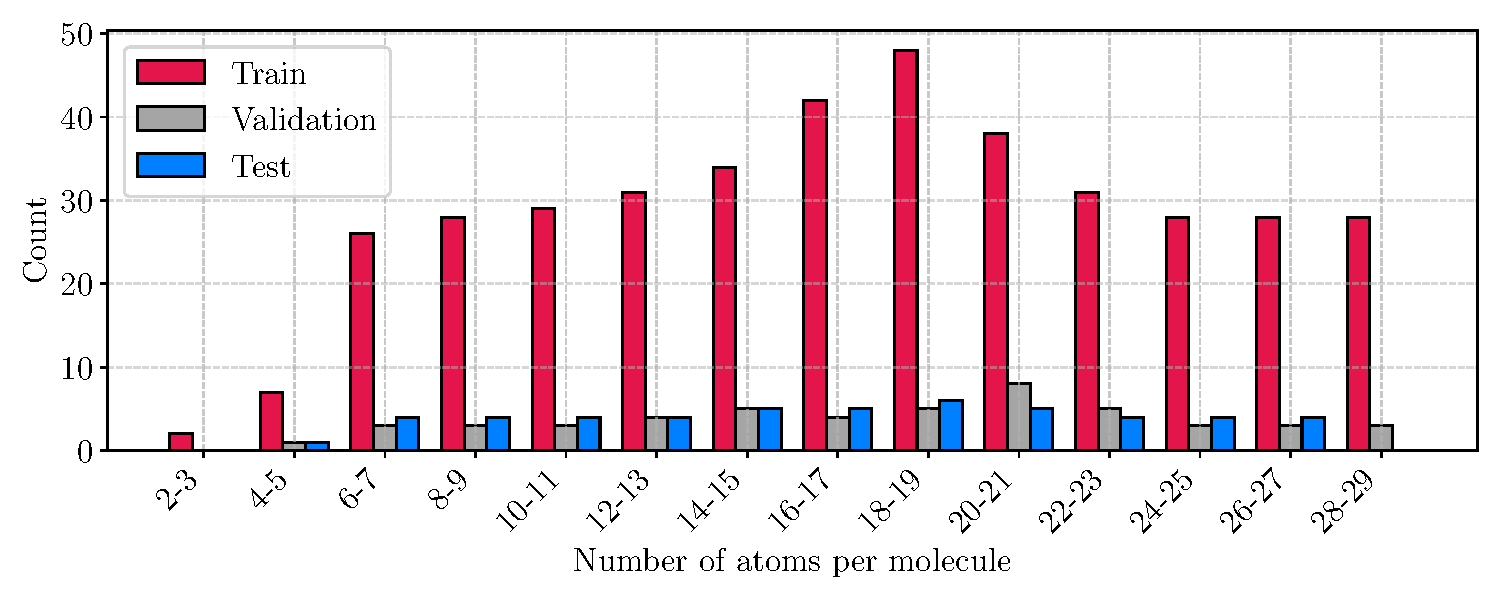
\includegraphics[width=\textwidth]{../fig/application/strat_sample.pdf}
    \caption[Stratified sample of QM9 dataset]{Stratified sample of QM9 dataset by number of atoms per molecule for each set.}
    \label{fig:sample_QM9}
\end{figure}
We sample 500 molecules from the QM9 set in a stratified manner and additionally ensure ample representation for various molecule sizes. Therefore, compared to the actual distribution seen in \autoref{fig:method_qm9_overview}, the representation of molecules with 6 to 13 and 24 to 29 atoms per molecule is increased. This results in the distribution for the train, validation and test sets shown in \autoref{fig:sample_QM9}. Once again the train / validation / test split is 80\% / 10\% / 10\%.\\

Zero-shot predictions like those devised in the previous section aren't possible on the full dataset due to missing encoders/decoders for \ch{N}, \ch{F} and their respective interaction blocks. Therefore, we'll proceed directly to hyperparameter tuning. 
\subsection{Hyperparameter tuning}
\label{sec:qm9_full_isomers_hyp_tuning}
\begin{table}[H]
    \centering
    \caption[GNN on full QM9 dataset sample with full matrix loss]{GNN on full QM9 dataset sample using full matrix loss to train. Metrics on test set and corresponding hyperparameter settings for 10 best performing networks in terms of iterations.}
    \label{tab:qm9_full_further_runs} 
    \resizebox{\textwidth}{!}{
        \begin{tabular}{l
                        S[table-format=2.1(2)]
                        S[table-format=-4(2)]
                        S[table-format=-1.3(2)]
                        S[table-format=1.3(1)]
                        S[table-format=1.4(1)]}
            \toprule
            Mean metrics:                 & {Iterations / 1} & {$\Delta E_\text{HF}$ / $\unit{\hartree}$}  & {$\delta E_\text{HF}$ / 1} & {DIIS error / $\unit{\hartree}$} & {RMSE / $\unit{\hartree}$} \\
            \midrule
            \bottomrule
        \end{tabular}
    }
        \resizebox{\textwidth}{!}{
        \begin{tabular}{lrrrrrrrrrr}
        \toprule
        Parameters & $\text{GNN}^{\text{Full}}_\text{f. 0}$ & $\text{GNN}^{\text{Full}}_\text{f. 1}$ & $\text{GNN}^{\text{Full}}_\text{f. 2}$ & $\text{GNN}^{\text{Full}}_\text{f. 3}$ & $\text{GNN}^{\text{Full}}_\text{f. 4}$ & $\text{GNN}^{\text{Full}}_\text{f. 5}$ & $\text{GNN}^{\text{Full}}_\text{f. 6}$ & $\text{GNN}^{\text{Full}}_\text{f. 7}$ & $\text{GNN}^{\text{Full}}_\text{f. 8}$ & $\text{GNN}^{\text{Full}}_\text{f. 9}$ \\
        \midrule

        \bottomrule
        \end{tabular}
        }
\end{table}

\TODO{Add graphic with distribution of iterations on testset (maybe sort by small - medium - large mols)}
\subsection{Evalutation \& Conclusion}
\label{sec:qm9_full_isomers_conclusion}

\begin{table}[H]
    \centering
    \caption[Models compared to \textsc{PySCF} and $\overline{P}$ schemes - full QM9 dataset]{Comparison of different models employing \textsc{PySCF} and $\overline{P}$ guessing schemes on the full QM9 dataset. Here, $\overline{P}$ is computed block-wise across all molecules by averaging over each \ch{C}, \ch{O}-\ch{H}, \dots block.
}
    \label{tab:qm9_full_test_overview}
    \resizebox{\textwidth}{!}{
        \begin{tabular}{l
                        S[table-format=2.1(1.1)]
                        S[table-format=-3.4(3)]
                        S[table-format=-1.6(1.1)]
                        S[table-format=1.3(1.1)]
                        S[table-format=1.4(1.1)]}
                        \toprule
                        Mean metrics:                 & {Iterations / 1} & {$\Delta E_\text{HF}$ / $\unit{\hartree}$}  & {$\delta E_\text{HF}$ / 1} & {DIIS error / $\unit{\hartree}$} & {RMSE / $\unit{\hartree}$} \\
                        \midrule
                        % &&&&&\\
                        $\overline{P}$                & 17(3)            & -800(200)     & -0.52(2)    & 0.11(2) & 0.014(2)  \\
                        \texttt{1-e}                  & 19(3)            & -225(4)    & -0.124(3)    & 0.122(15) & 0.16(12)  \\
                        \texttt{vsap}                 & 14(2)            & -4.8419(4) & -0.002665(19)& 0.024(3)  & 0.0106(14)\\
                        \texttt{atom}                 & 16(2)            & -14.0(9)   & -0.0077(5)   & 0.039(7)  & 0.015(2)  \\
                        \texttt{minao}                & \textbf{11.1(11)}& \textbf{2.86(2)} & \textbf{0.001577(0)}& 0.081(12) & 0.017(3)  \\
                        \bottomrule
                    \end{tabular}
    }
\end{table}
Another notable finding emerges when contrasting the full dataset results for $\overline{P}$ with those from the isomer only runs. Although the average number of iterations remained essentially unchanged (only their spread increased for the more diverse dataset) the DIIS error in the full dataset case is an order of magnitude higher. This increase is unsurprising given the broader chemical variety and the block-wise averaging inherent to $\overline{P}$. Crucially, it underscores that DIIS error and iteration count are largely uncorrelated.

\section{Lost Tweaks}
\label{sec:lost_tweaks}
\TODO{Optionally: Write about stuff that did not really make it }
